% !TEX root = ../thesis.tex
% simulation processes and execution
% @author Tobias Wulf
%

\section{Simulationsprozesse und Ausführung}\label{sec:sim-pro}


\subsection{Sensor-Array-Simulation}\label{sub:sensor-array-pro}


\begin{figure}[tbph]
	\centering
	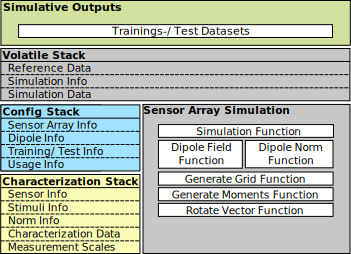
\includegraphics[width=0.7\linewidth]{chapters/images/3-SW-E-OExp/Blockschema_Sensor-Array}
	\caption[Blockschema Einbindung der Sensor-Array-Simulation]{Blockschema Einbindung der Sensor-Array-Simulation}
	\label{fig:blockschemasensor-array}
\end{figure}


\clearpage


\begin{figure}[tbph]
	\centering
	\includegraphics[width=\linewidth]{chapters/images/3-SW-E-OExp/Sensor-Array-Simulation}
	\caption[Sensor-Array-Simulation Prozessansicht]{Sensor-Array-Simulation Prozessansicht}
	\label{fig:sensor-array-simulation}
\end{figure}


\clearpage


\subsection{Gauß-Prozess-Regression}\label{sub:gpr-pro}


\paragraph{Trainingsphase}\label{par:gpr-training-pro}$~$\\


\begin{figure}[tbph]
	\centering
	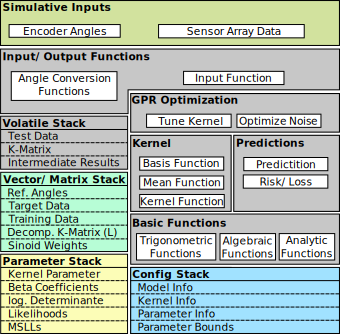
\includegraphics[width=0.7\linewidth]{chapters/images/3-SW-E-OExp/Blockschema_Trainingsphase}
	\caption[Blockschema Trainingsphase Regression]{Blockschema Trainingsphase Regression}
	\label{fig:blockschematrainingsphase}
\end{figure}


\clearpage


\begin{figure}[tbph]
	\centering
	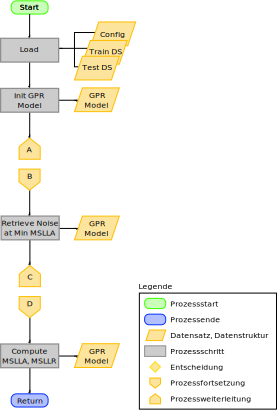
\includegraphics[width=.8\linewidth]{chapters/images/3-SW-E-OExp/GPR_Optimization}
	\caption[Regressionsoptimierung/ -Generalisierung Prozessansicht]{Regressionsoptimierung/ -Generalisierung Prozessansicht}
	\label{fig:gproptimization}
\end{figure}


\clearpage


\begin{figure}[htbp]
	\centering
	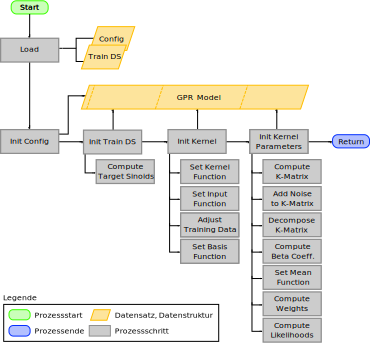
\includegraphics[width=0.7\linewidth]{chapters/images/3-SW-E-OExp/GPR_Initialization}
	\caption[Regressionsinitialisierung Prozessansicht]{Regressionsinitialisierung Prozessansicht}
	\label{fig:gprinitialization}
\end{figure}


\clearpage


\begin{figure}[tbph]
	\centering
	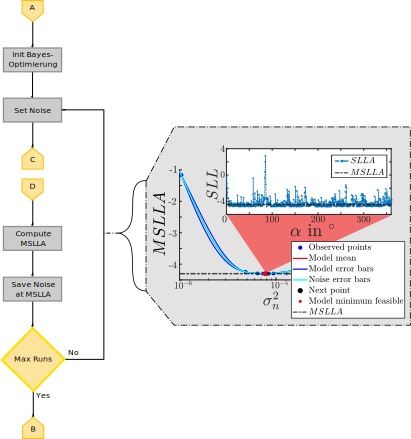
\includegraphics[width=0.85\linewidth]{chapters/images/3-SW-E-OExp/Noise_Optimization}
	\caption[Rauschniveauoptimierung Prozessansicht]{Rauschniveauoptimierung Prozessansicht}
	\label{fig:noiseoptimization}
\end{figure}


\clearpage


\begin{figure}[tbph]
	\centering
	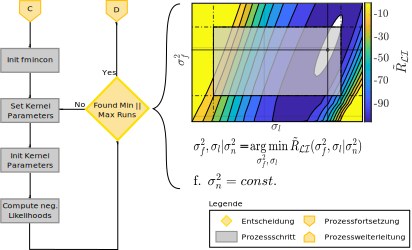
\includegraphics[width=0.8\linewidth]{chapters/images/3-SW-E-OExp/Kernel_Tuning}
	\caption[Regressionsparameteroptimierung Prozessansicht]{Regressionsparameteroptimierung Prozessansicht}
	\label{fig:kerneltuning}
\end{figure}


\clearpage


\paragraph{Arbeitsphase}\label{par:gpr-work-pro}$~$\\


\begin{figure}[tbph]
	\centering
	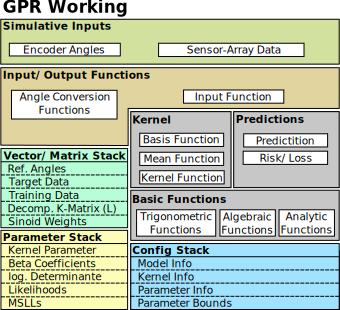
\includegraphics[width=0.7\linewidth]{chapters/images/3-SW-E-OExp/Blockschema_Workphase}
	\caption[Blockschema Arbeitsphase Regression]{Blockschema Arbeitsphase Regression}
	\label{fig:blockschemaworkphase}
\end{figure}

